% document formatting
\documentclass[10pt]{article}
\usepackage[utf8]{inputenc}
\usepackage[left=1in,right=1in,top=1in,bottom=1in]{geometry}
\usepackage[T1]{fontenc}
\usepackage{xcolor}

% math symbols, etc.
\usepackage{amsmath, amsfonts, amssymb, amsthm}

% lists
\usepackage{enumerate}

% images
\usepackage{graphicx} % for images

% code blocks
\usepackage{minted, listings} 

% verbatim greek
\usepackage{alphabeta}

\graphicspath{{./assets/images}}

\newcommand{\solution}{\textbf{Solution:}} 
\newcommand{\example}{\textbf{Example: }}

\title{EC ENGR 102 Week 3}

\author{Aidan Jan}
\date{\today}

\begin{document}
\maketitle

\subsection*{Memory}
\begin{itemize}
    \item A system has \textit{memory} if its output depends on past or future values of the input.  If the output depends only on present values of the input, the system is called \textit{memoryless}.
    \item e.g., $x(t) = A \cos(\omega t)$ is memoryless.
    \item $x(t) = \int_{-\infty}^t e^{-\tau^2} \text{d}\tau$ is not.
\end{itemize}

\subsection*{Invertibility}
\begin{itemize}
    \item A system is called \textit{invertible} if an input can always be exactly recovered from the output.  That is, a system $S$ is invertible if there exists an $S^{\text{inv}}$ such that
    \[x = S^{\text{inv}}(S(x))\]
    \item e.g., $y(t) = [x(t)]^2$ and $y(t) = \frac{\text{d}x(t)}{\text{d}t}$ are not invertible
    \item $y(t) = ax(t)$ for $a \neq 0$ is invertible.  Its inverse is $x(t) = \frac{1}{a} \cdot y(t)$.
\end{itemize}

\subsection*{System Impulse Response}
\begin{itemize}
    \item This lecture introduces time-domain analysis of systems, including the impulse response.  It also discusses linear time-invariant sysstems.  Topics include:
    \begin{itemize}
        \item Impulse response definition
        \item Impulse response of LTI systems
        \item The impulse response as a sufficient characterization of an LTI system
        \item Impulse response and the convolution integral
    \end{itemize}
    \item We've built a foundation on signal operations, signal models, and systems.  Today will be the first lecture where we present a new idea key to signals and systems: the impulse response.
    \item This impulse response will start us on the path to new concepts including convolution, Fourier series, and Fourier Transform
\end{itemize}

\section*{Impulse Response}
\subsection*{Why do we need the impulse response?}
\begin{itemize}
    \item In real life, we often do not have the luxury of knowing exactly what $S$ is, or perhaps we only know it imperfectly.  And even if we did know it, it could take on a very complicated form.
    \item The \textit{impulse response} is a characterization of the system that, for linear time-invariant systems, \textit{enables to calculate the output for \textbf{any} input}.  In this manner, it is a full time-domain description of the system.
\end{itemize}
\subsection*{Impulse Response Computation}
\[h(t) = H(\delta(t))\]
\begin{center}
    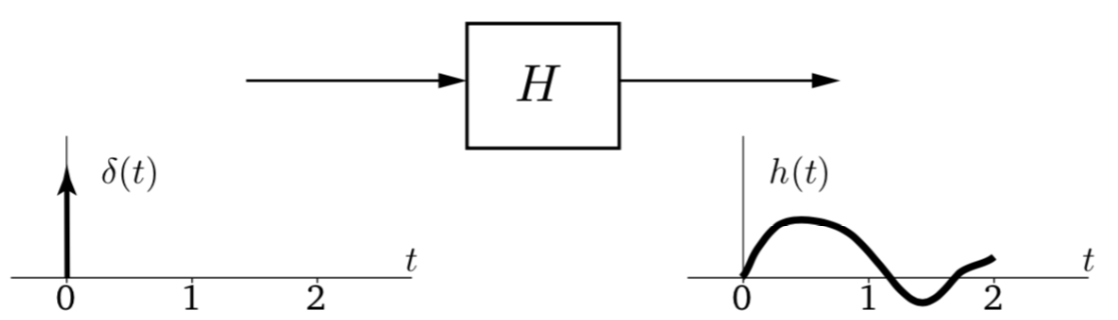
\includegraphics[scale=0.6]{W3_1.png}
\end{center}
\begin{itemize}
    \item In this case, our input signal is $x(t) = \delta(t)$, and our output is $y(t) = h(t)$.
\end{itemize}

\subsection*{Impulse response formal vs time invariant notation}
\underline{Formal:}
\begin{align*}
    y(t) &= H(x(t)) \\
    h(t) &= H(\delta(t)) \\
    h(t , \tau) &= H(\delta(t - \tau))
\end{align*}
\underline{Time-invariance:}
\begin{align*}
    h(t) &= H(\delta(t)) \\
    [FILL]
\end{align*}
\begin{center}
    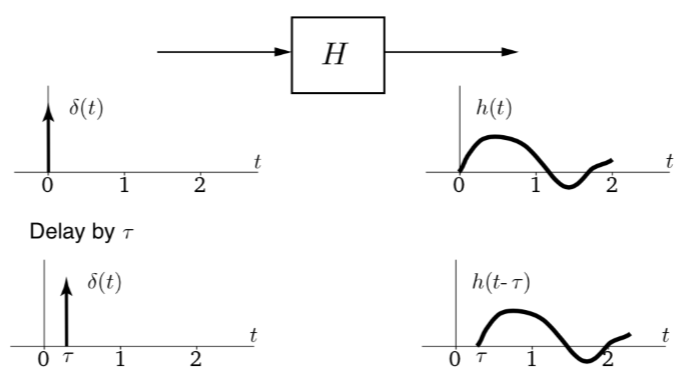
\includegraphics[scale=0.9]{W3_2.png}
\end{center}


\subsection*{A word on "t" in this formula}
\[h(t) = H(\delta(t))\]
In the above equation, the two $t$'s are NOT the same.
\begin{itemize}
    \item You cannot say $h(2) = H(\delta(2))$.
    \item The $t$ on the right is an independent variable that defines the input.
    \item The $t$ on the left is an independent variable that defines the output.
\end{itemize}
We can show this by making $h(t)$ the unit step function.  $h(2)$ would return 1, while $\delta(2)$ would return 0.

\subsection*{Extended Linearity}
Recall that a system, $H$, is linear if for $y_n = H(x_n)$ where $n$ is a subscript denoting different signals, and $a_n$ are constants, we have that:
\[\sum_n a_n y_n = H\left(\sum_n a_n x_n\right)\]
i.e., it has both homogeneity and superposition.  Thus, summation and the system operator can be interchanged.\\\\
In particular, this holds over integration (which is summation over infinitesimal intervals).  That is, if $y = H(x)$, then:
\[\int_{-\infty}^\infty a(\tau) y(t - \tau) \text{ d} \tau = H\left(\int_{-\infty}^\infty a(\tau) x(t - \tau) \text{ d}\tau\right)\]

\subsection*{Important fact about the impulse response}
\textbf{FACT:} If H is an LTI (linear time-invariant system) with impulse response
\[h(t) = H(\delta(t))\]
then we can calculate $H(x(t))$ for ANY $x(t)$ \textbf{\underline{IF}} we know $h(t)$.
\begin{itemize}
    \item Said differently, it is completely characterized by $h(t)$.  
    \item I can calculate $y(t)$ for \underline{any} $x(t)$ as long as I know $h(t)$.
\end{itemize}

\subsubsection*{Derivation of this fact}
Approach: write $x(t)$ in terms of $\delta(\tau)$'s.\\
Suppose $t = 0,\: x(0)$.
\[x(\tau) \cdot \delta(\tau) = x(0) \cdot \delta(\tau)\]
If we integrate this using the sampling property, we get $x(0)$.\\\\
If we now want to know what the value is at $x = 3$, then we do $t = 3,\:x(3)$.
\[x(\tau) \cdot \delta(\tau - 3) = x(3) \cdot \delta(\tau - 3)\]
By integrating this, we get the result of $x(3)$.\\\\
Now let's consider the general case: $x(t)$.
\[x(\tau) \cdot \delta(\tau - t) = x(t) \cdot \delta(\tau - t)\]
If we integrate this equation, we get $x(t)$.  Therefore, by sending an impulse through the circuit at particular values of $\tau$, we can find the result of the circuit.
\begin{align*}
    \int_{-\infty}^\infty x(\tau) \cdot \delta(\tau - t) \text{d}\tau &= \int_{-\infty}^\infty x(t) \cdot \delta(\tau - t) \text{d}\tau\\
    &= x(t) \cdot \int_{-\infty}^\infty \delta(\tau - t) \text{d}\tau\\
    &= x(t)
\end{align*}
We get the following two cases:
\begin{align*}
    x(t) &= \int_{-\infty}^\infty x(\tau) \delta(\tau - t) \text{d}\tau \\
    x(t) &= \int_{-\infty}^\infty x(\tau) \cdot \delta(t - \tau) \text{d}\tau
\end{align*}
From these two cases, we can assert that $\tau = t$.

\subsection*{The Convolution Integral}
\begin{align*}
    y(t) &= H(x(t))\\
    &= H\left(\int_{-\infty}^\infty x(\tau) \delta(t - \tau) \text{d}\tau\right)\\
    &= \int_{-\infty}^\infty x(\tau) H(\delta(t - \tau)) \text{d}t \hspace{2cm} \text{ this is possible since $H$ is linear}\\
    &= \int_{-\infty}^\infty x(\tau) \cdot h(t - \tau) \text{d}\tau \hspace{2cm} \text{H is time invariant.}
\end{align*}
If we now set the output to this function,
\[y(t) = \int_{-\infty}^\infty x(\tau) h(t - \tau) \text{d}\tau\]
This is called the "Convolution", or "Convolution integral".

\subsection*{Examples of computing the impulse response}
To find the impulse response,
\begin{enumerate}
    \item Set $x(t)$ to $\delta(t)$.
    \item We compute the system's output, $h(t) = H(\delta(t))$
\end{enumerate}
~\\
\underline{Example 1:}
What is the impulse response of $y(t) = \int_{-\infty}^t x(\tau) \text{d}\tau$?\\\\
\solution\\
It is the unit step function!
\begin{align*}
    h(t) &= \int_{-\infty}^t \delta(t) \text{d}\tau\\
    &= u(t)
\end{align*}
Note that $y(t) = \int_{-\infty}^\infty x(\tau) u(t - \tau) \text{d}\tau$, the convolution integral, is equal to the original $y(t)$ equation!\\\\
\underline{Example 2:}
\[y(t) = x(t - \alpha)\]
\solution\\
To find the impulse response, we apply the substitutions as described above:
\[h(t) = \delta(t - \alpha)\]

Looking at the convolution integral,
\begin{align*}
    y(t) &= \int_{-\infty}^\infty x(\tau) \cdot h(t - \tau) \text{d}\tau\\
    &= \int_{-\infty}^\infty x(\tau) \cdot \delta(t - T - \alpha) \text{d}\tau\\
    &= x(t - \alpha)
\end{align*}

\section*{Convolutions}
\subsection*{Intuition of what is going on in a convolution}
\begin{center}
    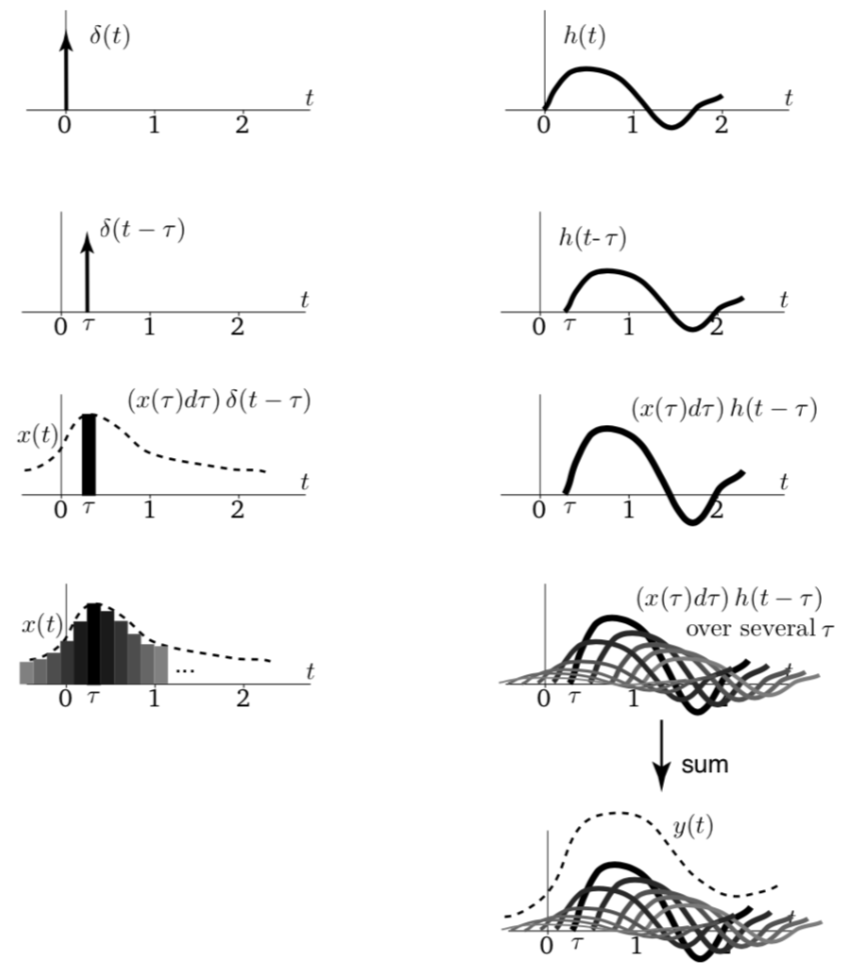
\includegraphics[scale=0.6]{W3_3.png}
\end{center}
Consider the convolution integral:
\[y(t) = \int_{-\infty}^\infty x(\tau) h(t - \tau) \text{d}\tau\]
Consider each graph on the left of the image as $x(t)$ (input), and the graph on the right of the image $y(t)$ (output).
\[x(t) \longrightarrow \boxed{H} \longrightarrow y(t)\]
The first two rows should be intuitive.  Input passes through function $H$ and returns the output.  The second row shows a time shift.\\\\
For the third row, write the interal as a riemann sum:
\begin{align*}
    x(t) &= \int_{-\infty}^\infty x(\tau) \delta(t - \tau) \text{d}\tau\\
    &= \sum_{n = -\infty}^\infty x(n \cdot \Delta \tau) \cdot \Delta \tau \cdot \delta(t - n \Delta \tau)
\end{align*}
One term out of the summation would be:
\[x(\Delta \tau) \cdot \Delta \tau \cdot \delta(t - \Delta \tau)\]
The first part of the formula ($x(\Delta \tau) \cdot \Delta \tau$) represents the area of the rectangle (highlighted on the left graph).  $\Delta \tau$ is the width, $x(\Delta \tau)$ is the height.  The remaining part ($\delta(t - \Delta \tau)$) is the time shift present on the right side.
This equation \textit{can} be thought as:
\begin{align*}
    & x(\Delta \tau) \cdot \Delta \tau \cdot \delta(t - \Delta \tau)\\
    &= H(\text{area} \cdot \delta(t - \Tau))\\
    &= \text{area} \cdot H(\delta(t - \tau))\\
    &= \text{area} \cdot h(t - \tau)
\end{align*}
\begin{itemize}
    \item We scale by the area of the rectangle because the height of the function $H$.  Since these are impulse responses, it makes sense that they are scaled.
\end{itemize}
The fourth row represents the graph with all of the terms of the riemann sum, which sum to the final function $y(t)$.
The \textit{convolution} essentially takes in an input signal, divides it into an infinite amount of scaled impulse responses (approximated by riemann sum), and sums the output for every impulse to find the output signal.
\begin{itemize}
    \item Notice: this allows you to pass an input signal (of your choosing) through a black box, and know the exact output signal.
\end{itemize}

\subsection*{Notation of Convolution}
\[y(t) = \int_{-\infty}^\infty x(\tau) h(t - \tau) \text{d}\tau\]
(This is a mathematical expression; the $t$ on both sides are the same, unlike last time.)\\
\example\\
\[y(5) = \int_{-\infty}^\infty x(\tau) h(5 - \tau) \text{d}\tau\]
\textbf{Notation:}
\[y(t) = (x * h)(t)\]
Convolution is denoted by the star ($*$).  This is the rigorous notation.\\\\
The convenient and common way is to write: $y(t) = x(t) * h(t)$.  However, this is bad because the $t$'s are not the same.  This adds confusion.\\\\
Additionally, in the block diagram, we write:
\[x(t) \longrightarrow \boxed{h(t)} \longrightarrow y(t)\]
also means the same thing.  A box with a variable in it represents convolution.

\subsection*{How to Compute Convolution: Flip and Drag}
\[y(t) = \int_{-\infty}^\infty x(\tau) h(t - \tau \text{d}\tau)\]
Let's break this integral down piece by piece.
\begin{itemize}
    \item The term $h(t - \tau)$, w.r.t., $t$, is the impulse response delayed to time $\tau$.
    \item However, our integral is over $\tau$ and so we should consider how $h$ varies with $\tau$.
    \item This term $h(t - \tau)$, w.r.t. $\tau$, tells us that we should first delay the signal to time $t$ and then reverse the signal.  This operation, which we colloquially call "flipping," is illustrated below.
\end{itemize}
\begin{center}
    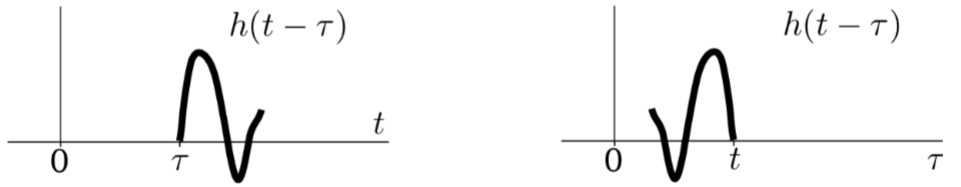
\includegraphics[scale=0.8]{W3_4.png}
\end{center}
\begin{itemize}
    \item Notice that the x-axis changes labels!
\end{itemize}
Next, convolution tells us to multiply $h(t - \tau)$, our flipped impulse response, with $x(\tau)$ and do it for all $\tau$.  This means we simply multiply $x(\tau)$ and $h(t - \tau)$ together pointwise.  This is illustrated below in red.
\begin{center}
    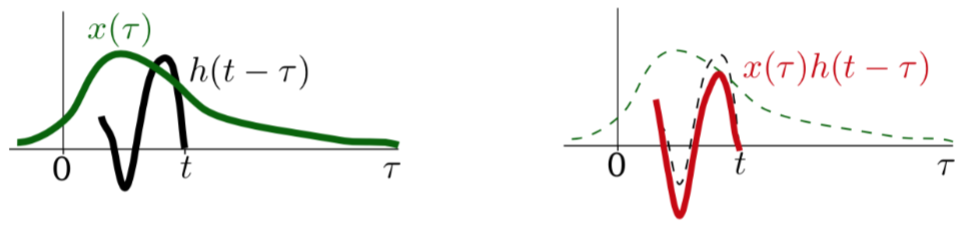
\includegraphics[scale=0.8]{W3_5.png}
\end{center}
Finally, to get $y(t)$ for this particular value of $t$, we integrate this curve over all $\tau$.  This is illustrated below.
\begin{center}
    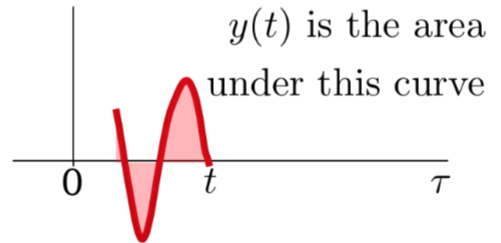
\includegraphics[scale=0.9]{W3_6.png}
\end{center}
Now, to get $y(t)$ for all values of $t$, we repeat this process, "dragging" $h(t - \tau)$ across different delays $t$.

\subsection*{Summary of the Flip and Drag Technique}
To calculate $y(t) = (x * h)(t)$:
(Convolutions are commutative, so $x$ and $h$ can be switched.  But, one can be thought of as the input and the other is the kernel.  Traditionally, $x$ is the input and $h$ is the impulse response.)
\begin{itemize}
    \item Flip (i.e., reverse in time) the impulse response.  This changes $h(\tau)$ to $h(-\tau)$.
    \item Begin to drag the reversed time response by some amount, $t$.  This results in $h(t - \tau)$.
    \item For a given $t$, multiply $h(t - \tau)$ pointwise by $x(\tau)$.  This produces $x(\tau) h(t - \tau)$.
    \item Integrate this product over $\tau$.  This produces $y(t)$ at this particular time $t$.
\end{itemize}
This technique is referred to as the "flip-and-drag" technique.
\begin{center}
    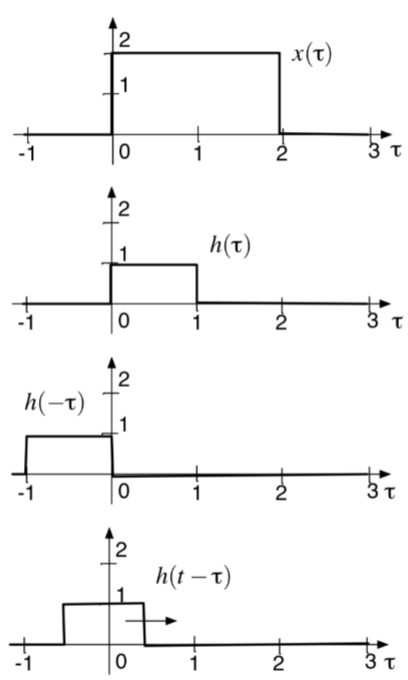
\includegraphics[scale=0.6]{W3_7.png}\\
\end{center}
\example\\
Consider the two rectangles given by $x(t)$ and $h(t)$.
\begin{center}
    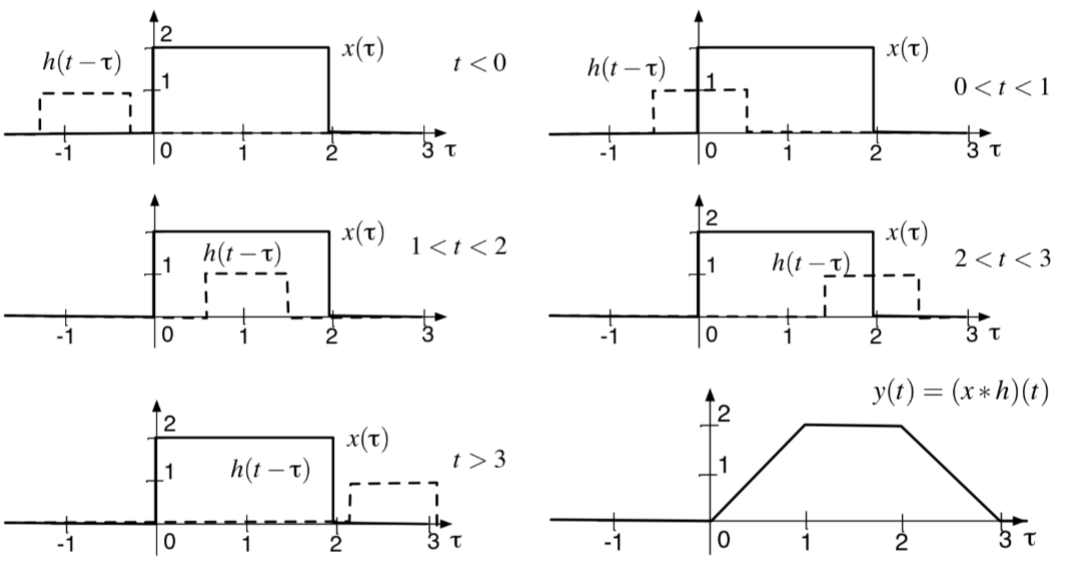
\includegraphics[scale=0.6]{W3_8.png}
\end{center}
\begin{itemize}
    \item When $t < 0$, the rectangles don't overlap.  Therefore, the product is 0, as seen in the bottom right graph.
    \item When $0 < t < 1$, we get parts of the rectangles overlapping, and as the overlap increases, the convolution increases.
    \begin{itemize}
        \item Suppose we use $t = 0.5$.  We have $y(t) = x(\tau) \times h(0.5 - \tau)$.  The left 0.5 of the $h(t)$ rectangle gives 0, while the right 0.5 of the $h(t)$ rectangle gives 2.  Integrating (finding average height) gives a height of 1.  Therefore, $y(0.5) = 1$ 
        \item If we did $t = 0.6$, we get $y(t) = x(\tau) \times h(0.6 - \tau)$.  That is, 0.6 of the rectangle is overlapping.  Then, the integral simplifies to $y(0.6) = (0.6 * 1 * 2 + 0.4 * 1 * 0) / 1 = 1.2$  Therefore, $y(0.6) = 1.2$.
    \end{itemize}
    \item When $1 < t < 2$, the rectangles are completely overlapping.  As a result, the average is going to be the product of the heights of both rectangles.  For example, $y(1.5) = 2$.
    \item When $2 < t < 3$, we get a similar case as $0 < t < 1$.  This time, since the overlap is decreasing with increasing $t$, the slope on the convolution is decreasing.
    \item Finally, if $t > 3$, the rectangles are no longer overlapping.  Therefore $y(t) = 0$.
\end{itemize}
Note: Convolutions can be done with pretty much any function!  Including impulses (which are basically rectangles with width 0)!

\subsection*{Causal Convolution}
In a causal system, $h(t) = 0$ for $t < 0$.  (Why?  Hint: what happens if $h(t) \neq 0$ for some $t < 0$?)\\\\
This means that $h(t - \tau) = 0$ if $\tau > t$.  Hence, there is no need to integrate if $\tau$ exceeds $t$, since $h(t - \tau) = 0$.  We can use this to simplify the convolution integral.
\begin{align*}
    y(t) &= \int_{-\infty}^\infty x(\tau) h(t - \tau) \text{d}\tau\\
    &= \int_{-\infty}^t x(\tau) h(t - \tau) \text{d}\tau
\end{align*}
This equation tells us that only past and present values of $x(\tau)$ contribute to $y(t)$.

\subsection*{Properties of Convolution}
\begin{itemize}
    \item \textbf{Commutativity}
    \[(x * h)(t) = (h * x)(t)\]
    \item \textbf{Associativity}
    \[(f * (g * h))(t) = ((f * g) * h)(t)\]
    \item \textbf{Distributivity}
    \[f * (g + h) = f * g + f * h\]
    \item \textbf{Linearity}
    \[h * (\alpha x_1 + \beta x_2) = \alpha(h * x_1) + \beta(h * x_2)\]
    \item \textbf{Time-invariance}
\end{itemize}

\subsubsection*{Proof of Commutativity}
\[x * h = h * x\]
\begin{align*}
    y(t) &= (x * h)(t) \\
    &= \int_{-\infty}^\infty x(\tau) h(t - \tau) \text{d}\tau\\
\intertext{Let $\tau' = t - \tau$.  Then, $\tau = t - \tau'$.  Also, $\text{d}\tau' = -\text{d}\tau$, and the bounds switch to $\infty \rightarrow -\infty$}
    &= \int_{-\infty}^\infty h(\tau')x(t - \tau') \text{d}\tau'\\
    &= (h * x)(t)
\end{align*}
Therefore, convolutions are commutative.
\end{document}